\documentclass[10pt, spanish]{beamer}

% --- Paquetes ---
\usepackage[utf8]{inputenc}
\usepackage[spanish]{babel}
\usepackage{graphicx}
\usepackage{amsmath}
\usepackage{amsfonts}
\usepackage{amssymb}
\usepackage{tikz}
\usetikzlibrary{shapes.geometric, arrows, positioning}

% --- Configuración de Tema ---
\usetheme{Madrid}
\usecolortheme{whale}
\setbeamercover{transparent}

% --- Metadatos ---
\title[Futbolito en VHDL]{Diseño e Implementación de un Sistema de Videojuego ``Futbolito'' sobre FPGA}
\subtitle{Proyecto de Arquitectura de Computadoras / Sistemas Digitales}
\author[Nombre del Autor]{Tu Nombre \\ \small Asesor: Nombre del Asesor}
\institute[Universidad]{Nombre de la Institución}
\date{\today}

% --- Estilos de Diagramas ---
\tikzstyle{block} = [rectangle, draw, fill=blue!20, text width=5em, text centered, rounded corners, minimum height=2em]
\tikzstyle{line} = [draw, -latex']

\begin{document}

% --- Portada ---
\begin{frame}
    \titlepage
\end{frame}

% --- Introducción ---
\begin{frame}{Introducción y Objetivos}
    \begin{columns}
        \begin{column}{0.6\textwidth}
            El proyecto consiste en el desarrollo de un videojuego interactivo de foosball (Futbolito) implementado directamente en hardware.
            \vspace{0.5cm}
            \textbf{Objetivos Principales:}
            \begin{itemize}
                \item Implementación de un controlador VGA (640x480).
                \item Procesamiento de gráficos en tiempo real.
                \item Gestión de lógica de juego mediante procesos concurrentes.
            \end{itemize}
        \end{column}
        \begin{column}{0.4\textwidth}
            \begin{figure}
                \centering
                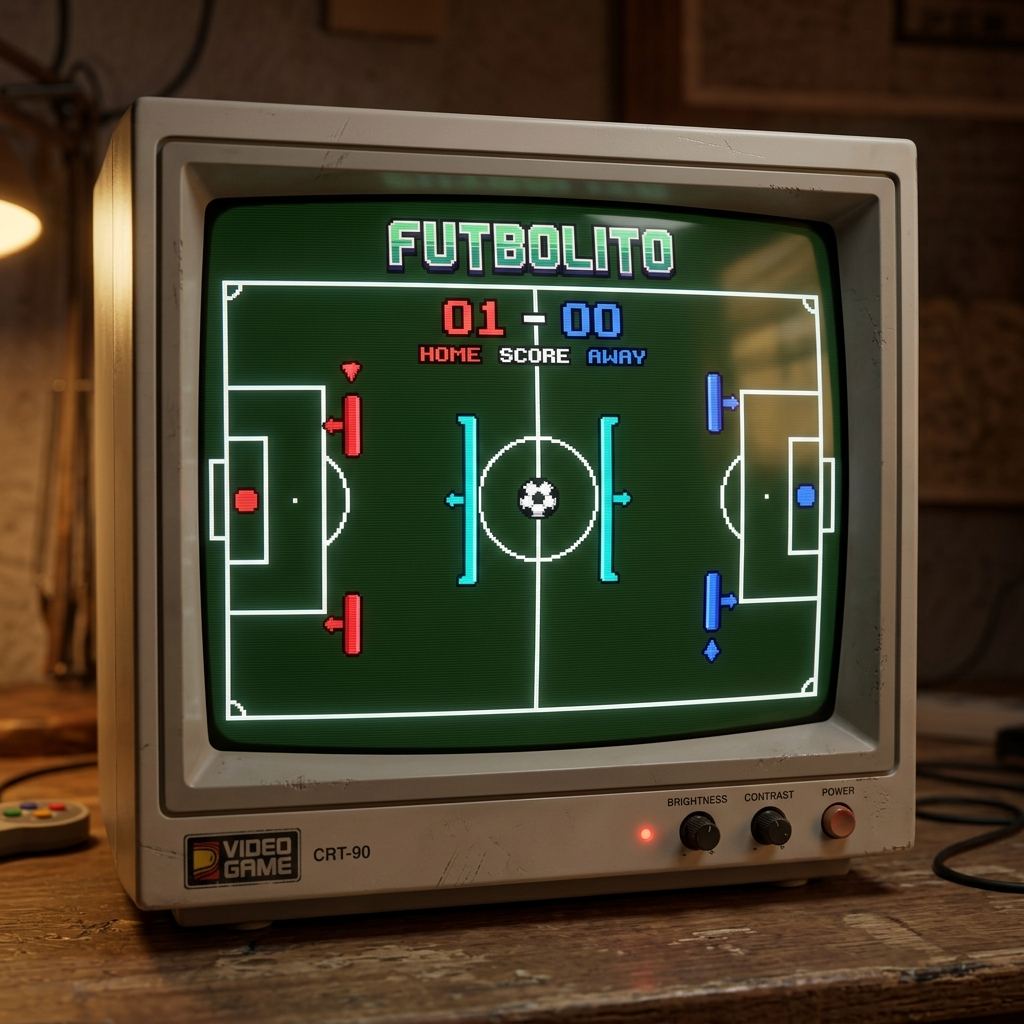
\includegraphics[width=\textwidth]{./assets/mockup_juego.png}
                \caption{Mockup conceptual}
            \end{figure}
        \end{column}
    \end{columns}
\end{frame}

% --- Arquitectura ---
\begin{frame}{Arquitectura del Sistema}
    \centering
    \begin{tikzpicture}[node distance = 2cm, auto]
        % Nodos
        \node [block] (clk) {Reloj 50\,MHz};
        \node [block, right of=clk, node distance=2.5cm] (pll) {Divisor / PLL 25\,MHz};
        \node [block, below of=pll, node distance=1.5cm] (top) {Top Level (top\_futbolito)};
        \node [block, below left of=top, node distance=2.5cm] (sync) {VGA Sync (vga\_sync)};
        \node [block, below right of=top, node distance=2.5cm] (game) {Game Logic (BALL)};
        \node [block, below of=game, node distance=1.5cm] (rom) {Ball ROM};
        
        % Líneas
        \path [line] (clk) -- (pll);
        \path [line] (pll) -- (top);
        \path [line] (top) -- (sync);
        \path [line] (top) -- (game);
        \path [line] (rom) -- (game);
    \end{tikzpicture}
    \vspace{0.3cm}
    \begin{itemize}
        \item Estructura jerárquica con modularización de funciones.
        \item Comunicación mediante señales de 10 bits para coordenadas de píxeles.
    \end{itemize}
\end{frame}

% --- Sincronización VGA ---
\begin{frame}{Sincronización de Video (VGA)}
    Se utiliza el estándar estándar \textbf{640x480 @ 60\,Hz}:
    \begin{itemize}
        \item \textbf{Timing Horizontal:} 800 ciclos de reloj por línea (640 activos).
        \item \textbf{Timing Vertical:} 525 líneas por cuadro (480 activas).
        \item \textbf{Salida:} DAC de video de la DE2-115 (pines H10, G8, B10, etc.).
    \end{itemize}
    \vfill
    \begin{block}{Divisor de Reloj}
        La señal de 50\,MHz de la FPGA se divide entre 2 para obtener los 25\,MHz necesarios por el estándar VGA.
    \end{block}
\end{frame}

% --- Lógica de Juego ---
\begin{frame}{Lógica de Juego y Colisiones}
    Implementado en el módulo \texttt{BALL.VHD}:
    \begin{description}
        \item[Movimiento Pelota:] Actualización de coordenadas $(X, Y)$ en cada \texttt{Vert\_sync}.
        \item[Colisiones:] Lógica booleana para detectar intersección de áreas:
            \[ \text{Ball\_on } \cap \text{ (Paddle\_on } \cup \text{ Defense\_on)} \]
        \item[Física:] Reflexión simple invirtiendo el vector \texttt{Ball\_X\_motion}.
    \end{description}
    \vfill
    \begin{exampleblock}{Entradas}
        Uso de pulsadores físicos (Keys/Pushbuttons) de la FPGA para controlar los porteros.
    \end{exampleblock}
\end{frame}

% --- Sprites y ROM ---
\begin{frame}{Generación de Sprites vía ROM}
    Para una apariencia más detallada del balón (16x16 píxeles):
    \begin{itemize}
        \item \textbf{Herramienta:} Script Python \texttt{img\_to\_vhdl.py} para convertir PNG a VHDL.
        \item \textbf{Memoria:} Capacidad de 256 palabras.
        \item \textbf{Prioridad de Dibujo:} El sprite tiene la máxima prioridad visual, usando un canal Alpha de 1 bit para transparencia.
    \end{itemize}
    \begin{center}
        \texttt{pixel\_coord} $\rightarrow$ \texttt{rom\_address} $\rightarrow$ \texttt{rom\_pixel\_data}
    \end{center}
\end{frame}

% --- Conclusiones ---
\begin{frame}{Conclusiones y Resultados}
    \begin{enumerate}
        \item \textbf{Modularidad:} El diseño jerárquico permite escalar el juego (añadir más defensas o efectos).
        \item \textbf{Hardware vs Software:} La implementación en hardware garantiza una latencia nula en la respuesta del video.
        \item \textbf{Recursos:} Uso eficiente de bloques de memoria (M9K) para el almacenamiento de sprites.
    \end{enumerate}
    \vfill
    \begin{center}
        \huge \textit{¿Preguntas?}
    \end{center}
\end{frame}

\end{document}
